\chapter{Numerische Methoden}

\section{Einleitung}

Mit den in Kapitel () eingeführten Bewegungsgleichungen fehlt uns nur noch die Numerik um die zeitliche Entwicklung eines Models aus
gegebene Anfangs- und Randbedingungen zu berechnen.
Für die numerische Lösung von partiellen Differentialgleichungen eignen sich eine Vielzahl an Methoden, für die Berechnung auf
der GPU-Architektur erweist sich aber insbesondere die Verwendung von Finite Differenzen  auf kartesischen Gittern
als sehr effektiv (siehe Kapitel ()).
Während die Finite Differenzen für die räumliche Diskretisierung verwendet werden, wird für die zeitliche Diskretisierung
das Runge-Kutta Verfahren 3. Ordnung benutzt.


\section{Finite Differenzen}
Zunächst soll eine kurze Einleitung in die Methode der Finite Differenzen gegeben werden.
Für eine ausführlichere Herleitung, auf welcher dieser Abschnitt beruht, sei  auf [Peric etc.] verwiesen (REWRITE).
Wir betrachten hier den eindimensionalen Fall einer stetig differenzierbare Funktion $f(x)$ (defi?), das Ziel ist es nun die Ableitungen

\begin{align}
\pdn[f]{x} \ , \ \pdn[^2f]{x^2}
\end{align}

mit einem möglichsten kleinen Fehler zu diskretisieren.
Betrachten wir die Funktion $f$ auf einem Intervall von 0 bis $L$, so können wir diese durch $N$ äquidistante Punkte $x_i; 0 seq i s 100$ approximieren (s.Abb.x).
Der Abstand zwischen zwei Punkten ergibt sich dann als $\Delta x = L/(N - 1)$.
Betrachten wir $f$ in der Umgebung des Punkt $x_i$ so können wir $f$ über eine Taylor-Entwicklung ausdrücken

\begin{align}
    f(x) = f(x_i) + \left(\pdn[f]{x} \right)_i (x - x_i) + \left(\pdn[^2f]{x^2}\right)_i \frac{(x-x_i)^2}{2!}
\end{align}

Nun haben wir die Möglichkeit $x$ durch $x_{i+1}$ oder $x_{i-1}$ zu ersetzen. Nach vernachlässigen von Termen größer zweiter Ordnung erhalten wir nach umstellen
\begin{align}
    \left(\pdn[f]{x}\right)_i &\approx \frac{f_{i+1} - f{i}}{\Delta x}\\
    \left(\pdn[f]{x}\right)_i &\approx \frac{f_{i} - f_{i-1}}{\Delta x}\\
    \left(\pdn[f]{x}\right)_i &\approx \frac{f_{i+1} - f_{i-1}}{2\Delta x}
\end{align}

\begin{figure}[!tpb]
  \centering
  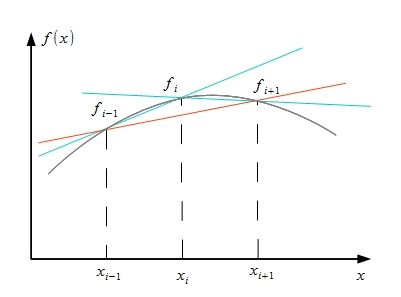
\includegraphics[width=0.6\textwidth]{gfx/numerik/fd_dummy.png}\label{fig:fd_schema}
  \caption{Approximation einer Funktion durch finite Differenznen}
\end{figure}

Die Approximation () enspricht für $dx>0$ der Definition der Ableitung und wird als Vorwärtsdifferenz bezeichnet,
während () als Rückwärtsdifferenz bezeichnet wird.
Die dritte Approximation () ergibt sich durch Mittelung über die ersten beiden Variante und wird als zentrierte Differenz bezeichnet.
Vergleicht man die grafische Darstellung der Terme in Abbildung () so sieht man hier bereits,
dass die zentrierte Differenz die Steigung der Funktion am Punkt $x_i$ exakter approximieren kann.


\paragraph{Lokaler Abschneidefehler}\mbox{}\\

Der Abschneidefelher $T_{ik}$ bezeichnet den lokalen Diskretisierungsfehler welcher durch die Approximation entsteht.
Die Berechnung erfolgt dur einsetzen
-beispielrechnung


\paragraph{Stabilitätsanalyse}\mbox{}\\

-beispiel erste abl dann zweit
-stabilität konstistenz - konvergenz etc
-verfahren höherer ordnung
-peclet zahl
-upwind schema


\section{Runge Kutta Verfahren}
Für die zeitliche Diskretierung wird ein Runge-Kutta Verfahren dritter Ordnung verwendet.
Ein Vorteil des Verfahrens dritter Ordnung ist die Stabilität gegenüber Oszillationen bei CFD-Problemen [QUOTE].
Allgemein wird bei der Herleitung

-warum ordnung 3
-runge kutta williamson etc
-stabilität
-fehler

\newpage

\section{Artificial Kompressibility}
bewegungsgleichungen
druckterm diskussion
exkurs laplace gleichung
beispiel rayleigh benard diskretisierung

